\documentclass[10pt,border=1pt]{standalone}
\usepackage[T1]{fontenc}
\usepackage{mathpazo}
\usepackage{amsmath,amssymb}
\usepackage{xcolor}
\usepackage{pgfplots}
\pgfplotsset{compat=1.18}
\usetikzlibrary{shapes.geometric,positioning,arrows.meta,calc}
\definecolor{okorange}{HTML}{E69F00}
\definecolor{oksky}{HTML}{56B4E9}
\definecolor{okgreen}{HTML}{009E73}
\definecolor{okblue}{HTML}{0072B2}
\definecolor{okverm}{HTML}{D55E00}
\definecolor{okpurple}{HTML}{CC79A7}
\colorlet{accent}{okverm}
\pgfplotsset{
  safenest/.style={
    tick label style={font=\footnotesize},
    label style={font=\small},
    title style={font=\small, align=left},
    legend style={font=\footnotesize, draw=none, fill=none, cells={anchor=west}},
    grid style={black!12, line width=0.3pt},
    axis line style={black!70, line width=0.4pt},
    tick style={black!70, line width=0.4pt},
    axis lines*=left,
  },
}
\newlength{\figwidth}
\tikzset{every node/.append style={execute at begin node={\hyphenpenalty=10000\exhyphenpenalty=10000\relax}}}
\setlength{\figwidth}{18.47cm}
\begin{document}
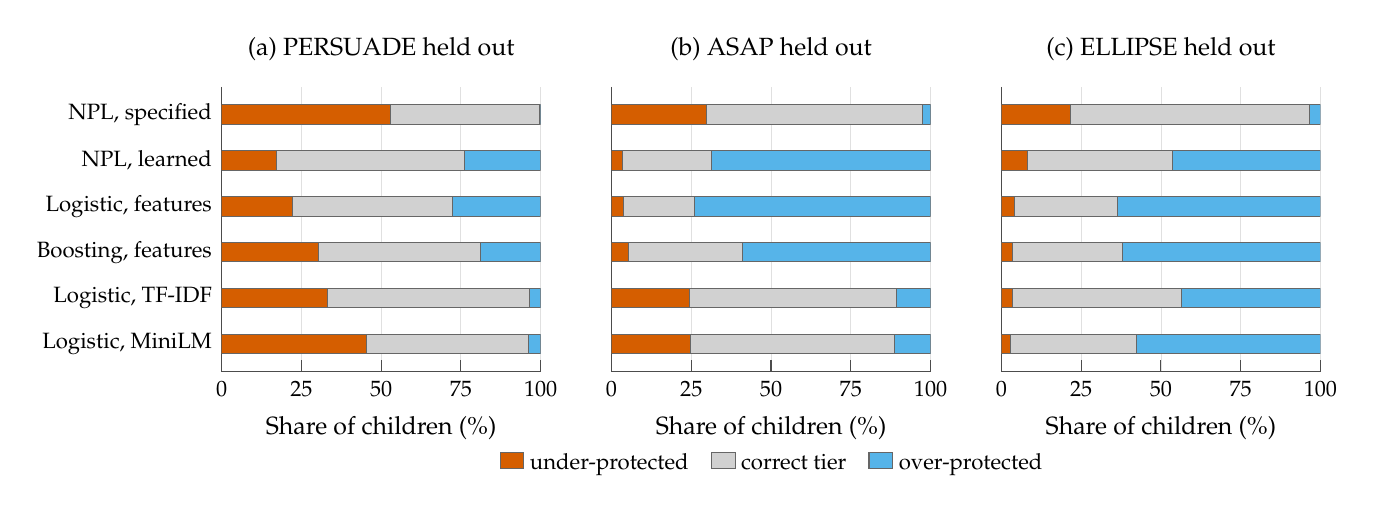
\begin{tikzpicture}
\begin{axis}[safenest, name=p1, 
  width=0.305\figwidth, height=52mm, scale only axis=false,
  xbar stacked, bar width=7pt, xmin=0, xmax=100, y dir=reverse,
  ytick={0,1,2,3,4,5}, yticklabels={{NPL, specified},{NPL, learned},{Logistic, features},{Boosting, features},{Logistic, TF-IDF},{Logistic, MiniLM}},
  enlarge y limits=0.12, xmajorgrids, xtick={0,25,50,75,100},
  xlabel={Share of children (\%)}, title={(a) PERSUADE held out},
]
\addplot[fill=accent, draw=black!60, line width=0.3pt] coordinates {(52.9,0) (17.2,1) (22.1,2) (30.3,3) (33.0,4) (45.4,5)};
\addplot[fill=black!18, draw=black!60, line width=0.3pt] coordinates {(46.8,0) (58.9,1) (50.1,2) (50.9,3) (63.6,4) (50.8,5)};
\addplot[fill=oksky, draw=black!60, line width=0.3pt] coordinates {(0.3,0) (23.9,1) (27.8,2) (18.8,3) (3.4,4) (3.8,5)};
\end{axis}
\begin{axis}[safenest, name=p2, at={($(p1.east)+(9mm,0)$)}, anchor=west,
  width=0.305\figwidth, height=52mm, scale only axis=false,
  xbar stacked, bar width=7pt, xmin=0, xmax=100, y dir=reverse,
  ytick={0,1,2,3,4,5}, yticklabels={},
  enlarge y limits=0.12, xmajorgrids, xtick={0,25,50,75,100},
  xlabel={Share of children (\%)}, title={(b) ASAP held out},
]
\addplot[fill=accent, draw=black!60, line width=0.3pt] coordinates {(29.6,0) (3.3,1) (3.7,2) (5.2,3) (24.5,4) (24.6,5)};
\addplot[fill=black!18, draw=black!60, line width=0.3pt] coordinates {(67.9,0) (27.9,1) (22.2,2) (35.9,3) (64.9,4) (64.1,5)};
\addplot[fill=oksky, draw=black!60, line width=0.3pt] coordinates {(2.5,0) (68.8,1) (74.1,2) (58.9,3) (10.7,4) (11.4,5)};
\end{axis}
\begin{axis}[safenest, name=p3, at={($(p2.east)+(9mm,0)$)}, anchor=west,
  width=0.305\figwidth, height=52mm, scale only axis=false,
  xbar stacked, bar width=7pt, xmin=0, xmax=100, y dir=reverse,
  ytick={0,1,2,3,4,5}, yticklabels={},
  enlarge y limits=0.12, xmajorgrids, xtick={0,25,50,75,100},
  xlabel={Share of children (\%)}, title={(c) ELLIPSE held out},
]
\addplot[fill=accent, draw=black!60, line width=0.3pt] coordinates {(21.6,0) (8.2,1) (4.2,2) (3.6,3) (3.6,4) (2.9,5)};
\addplot[fill=black!18, draw=black!60, line width=0.3pt] coordinates {(75.0,0) (45.3,1) (32.3,2) (34.4,3) (52.9,4) (39.5,5)};
\addplot[fill=oksky, draw=black!60, line width=0.3pt] coordinates {(3.4,0) (46.5,1) (63.5,2) (62.0,3) (43.5,4) (57.7,5)};
\end{axis}
\node[anchor=north, font=\footnotesize] at ($(p2.south)+(0,-9mm)$) {%
  \tikz\fill[accent, draw=black!60] (0,0) rectangle (3mm,2mm);~under-protected\quad
  \tikz\fill[black!18, draw=black!60] (0,0) rectangle (3mm,2mm);~correct tier\quad
  \tikz\fill[oksky, draw=black!60] (0,0) rectangle (3mm,2mm);~over-protected};
\end{tikzpicture}
\end{document}
